\documentclass[12pt]{article}
\usepackage[spanish]{babel}
\selectlanguage{spanish}
\usepackage[utf8]{inputenc}
\usepackage{vmargin}
\usepackage{graphicx}
\setmargins{2.3cm}{1.3cm}{16.5cm}{23.2cm}{0pt}{1cm}{0pt}{2cm}
\title{Movimiento de Proyectiles en Gnuplot}
\author{Paulina Valenzuela Coronado}
\date{Marzo 2015}

\begin{document}
\maketitle
\section{Trayectoria de un Proyectil}
Cuando se lanza un objeto en presencia solamente de un campo gravitatorio,como el de la tierra, se observa que dicho objeto se eleva, alcanza una determinada altura y cae. Las ecuaciones vectoriales
que describen este tipo de movimientos son:  
entonces se cumple que:
\begin{center}
$\vec{r}= \vec{r}_0+ \vec{v}_0t+ \frac{1}{2} \vec{a}t^2$ 
\end{center}

Este movimiento ocurre en un plano y para su estudio se puede descomponer en un movimiento en la dirección horizontal y otro en la dirección vertical.
En la dirección horizontal, el movimiento es uniforme con velocidad constante y las ecuaciones que lo describen son: 
\begin{center}
$ x(t)= x_0 + v_0xt$
\end{center}
\begin{center}
$ V_x(t)= V_0x=cte$
\end{center}
Donde $x_0$ es la componente horizontal de la posición inicial y $V_0x$ es la componente horizontal del vector
velocidad inicial.En la dirección vertical, el movimiento es uniformemente acelerado, donde la aceleración es debida al campo gravitatorio. Las ecuaciones que lo describen son: 
\begin{center}
$y(t)=y_0+V_0t+\frac{1}{2}at^2$
\end{center}

donde $V_0$ es la componente vertical de la posición inicial, $x_0$ es la componente vertical de la velocidad
inicial y $a$ es la componente vertical de la aceleración. 
\section{Calcula el movimiento del proyectil}

Para esta actividad se nos proporciono un código fortran que calcula la posición al lanzar un proyectil. Al compilar y ejecutar el código, se pedía una velocidad inicial y un ángulo, después de esto obteniamos un archivo $.dat$ que contenia todas los datos de posición. Se uso este archivo para gráficar el movimiento en gnuplot.
Para modificar el programa dado y hacer que calcule y nos muestre el tiempo, vuelo y alcance del proyectil, se debe de agregar al código una serie de ecuaciones, estas son:
\begin{center}
$ t = \frac{2v_0 sin(0}{g}$
\end{center}
\begin{center}
$h = \frac{v_0^2 sin^2(0)}{2g}$
\end{center}
\begin{center}
$d = \frac{v_0^2}{g} sin(20)$
\end{center}


Teniendo estas ecuaciones, el programa este será capaz de calcular el tiempo, la altura y el alcance máximo.

\subsection{Código nuevo en Fortran}

\begin{verbatim}
Program Proyectilfinal
implicit none
real, parameter :: pi = 4.0*atan(1.0)
real :: v, a, t, h, r, a_grados
real, parameter :: g = 9.81
real :: x(2000),y(2000)
integer :: i
write (*,*) 'Enter angle of projectile (Real)'
read *, a_grados
write (*,*) 'Enter velocity of projectile (Real)'
read *, v
a = a_grados*pi/180.0
t = 2*v*sin(a)*(1/g)
h = v*v*sin(a)*sin(a)*(1/(2*g))
r = v*v*sin(2*a)*(1/g)
print * , 'Tiempo total de vuelo=' , t
print * , 'Altura máxima alcanzada=' , h
print * , 'Distancia máxima alcanzada=' , r
open(1, file='proy.dat')
do i=1,2000
t = (float(i)*0.01)
x(i) = v*cos(a)*t
y(i) = v*sin(a)*t - 0.5*g*t*t
write(1,*) x(i), y(i)
if (y(i)<0) exit
end do
close(1)
End Program Proyectilfinal
\end{verbatim}
\pagebreak
\subsection{Ejemplos}
Ángulo: $90^{\circ}$
\begin{center}
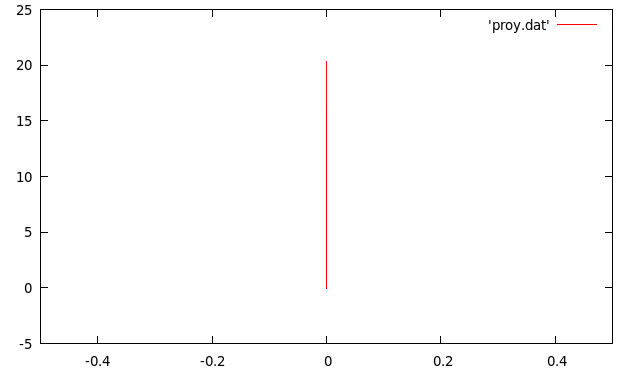
\includegraphics[scale=0.6]{Grafica90.png}
\end{center}

\begin{center}
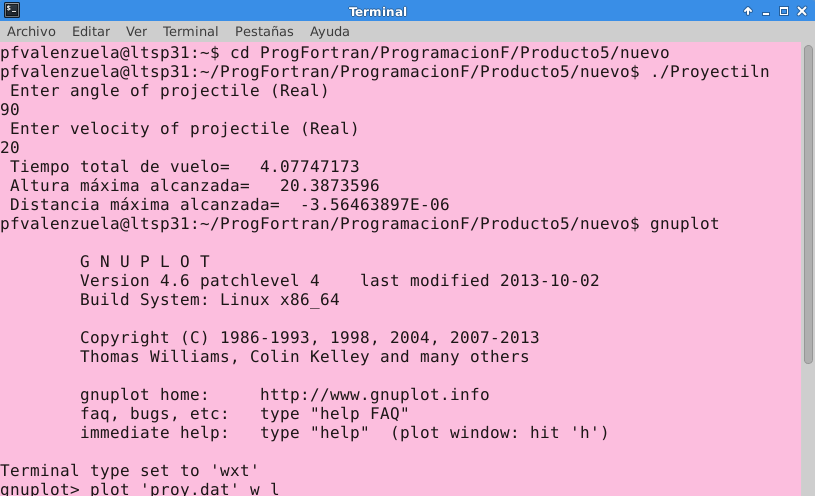
\includegraphics[scale=0.6]{Resultados90.png}
\end{center}

Ángulo: $0^{\circ}$
\begin{center}
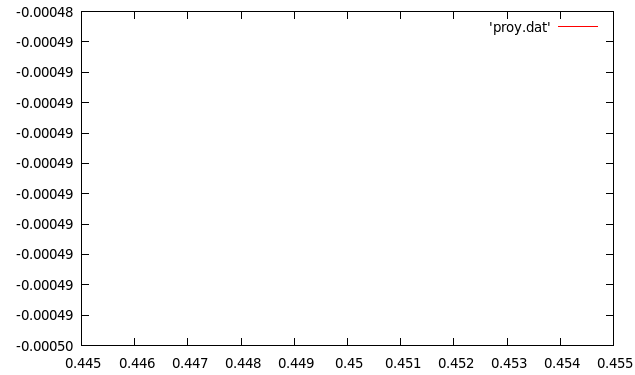
\includegraphics[scale=0.6]{Grafica0.png}
\end{center}

\begin{center}
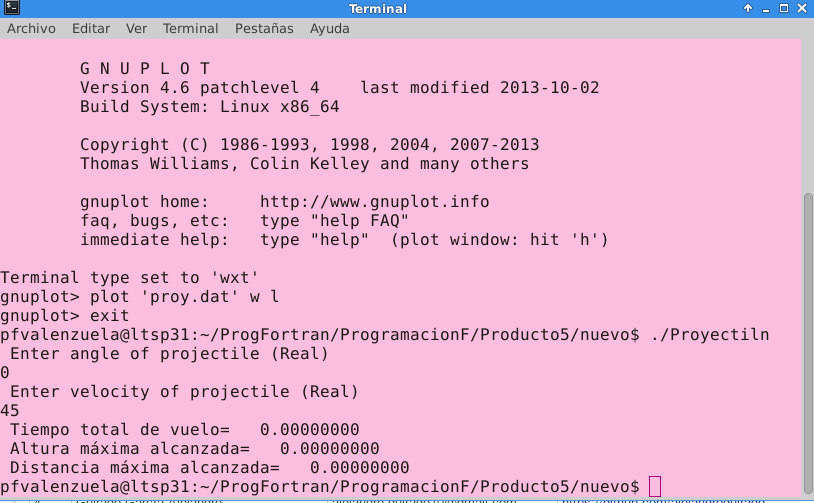
\includegraphics[scale=0.6]{Resultados0.png}
\end{center}


Ángulo: $60^{\circ}$
\begin{center}
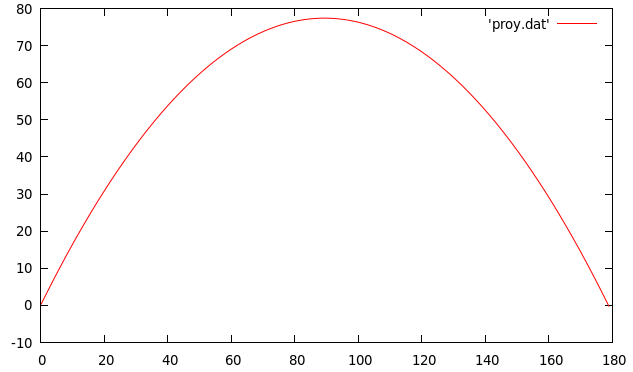
\includegraphics[scale=0.6]{Grafica60.png}
\end{center}

\begin{center}
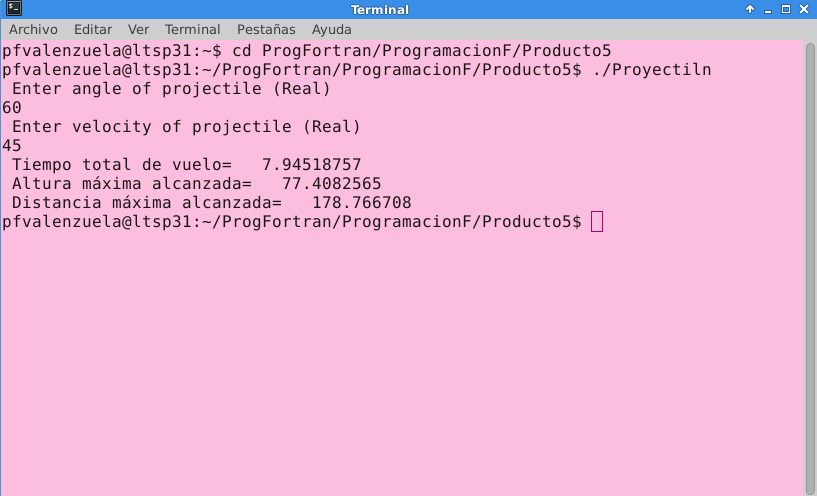
\includegraphics[scale=0.6]{Resultados60.png}
\end{center}


Ángulo:  $30^{\circ}$
\begin{center}
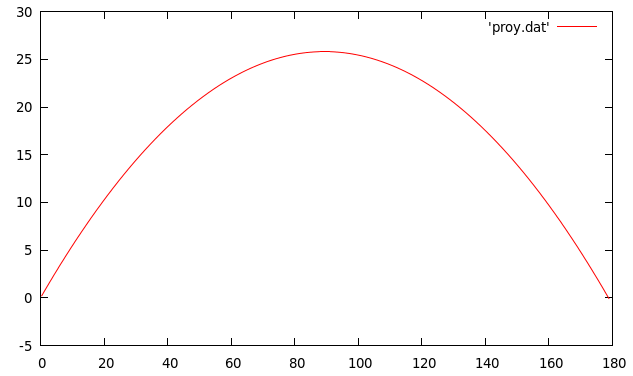
\includegraphics[scale=0.6]{Grafica30.png}
\end{center}

\begin{center}
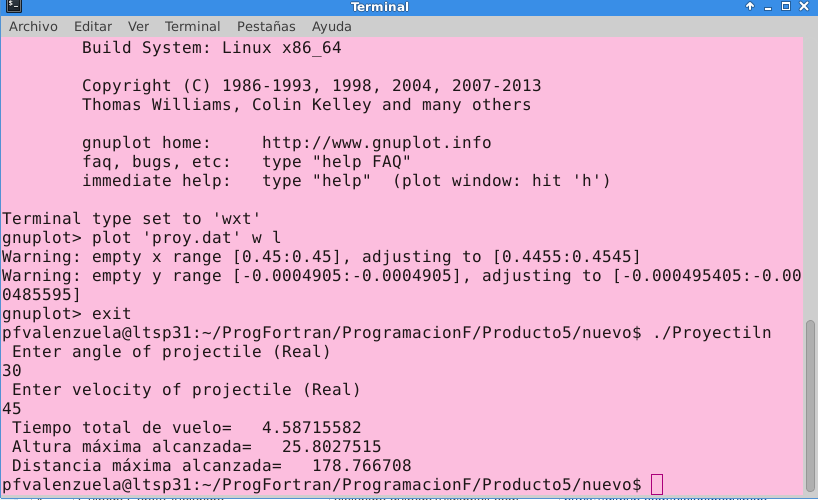
\includegraphics[scale=0.6]{Resultados30.png}
\end{center}


\end{document}